\documentclass{report}
\title{Efficient Planning for Sokoban with Answer Set Programming - A Case Study}
\author{Thomas Verweyen}
\date{\today}
\usepackage{listings}
\usepackage{graphicx}
\usepackage{titlesec}
\graphicspath{{./images/}}
\usepackage{color}
%\lstset{numbers=left,
%literate = {-}{-}1,
%basicstyle=\footnotesize,
%numbersep=5pt, backgroundcolor=\color{white},
%captionpos=b,keywordstyle=\color{blue},
%commentstyle=\color{green}}
\begin{document}
\maketitle
\renewcommand*\contentsname{Summary}
\tableofcontents
\section*{Abstract}
\chapter{Introduction}

\chapter{What is Sokoban}
\section{Background}
Sokoban is a logistic planning puzzle game from Japan. Sokoban was apparently created by Hiroyuki Imabayashi in 1981, and published by \textit{Thinking Rabbit} in 1982. Sokoban means warehouse person in japanese. The game has very simple rules but shows to be very complex for humans and for AI. This makes Sokoban a very interesting subject for research regarding planning problems.
\section{Rules} \label{IntroStr}
\begin{figure}[ht]
\centering
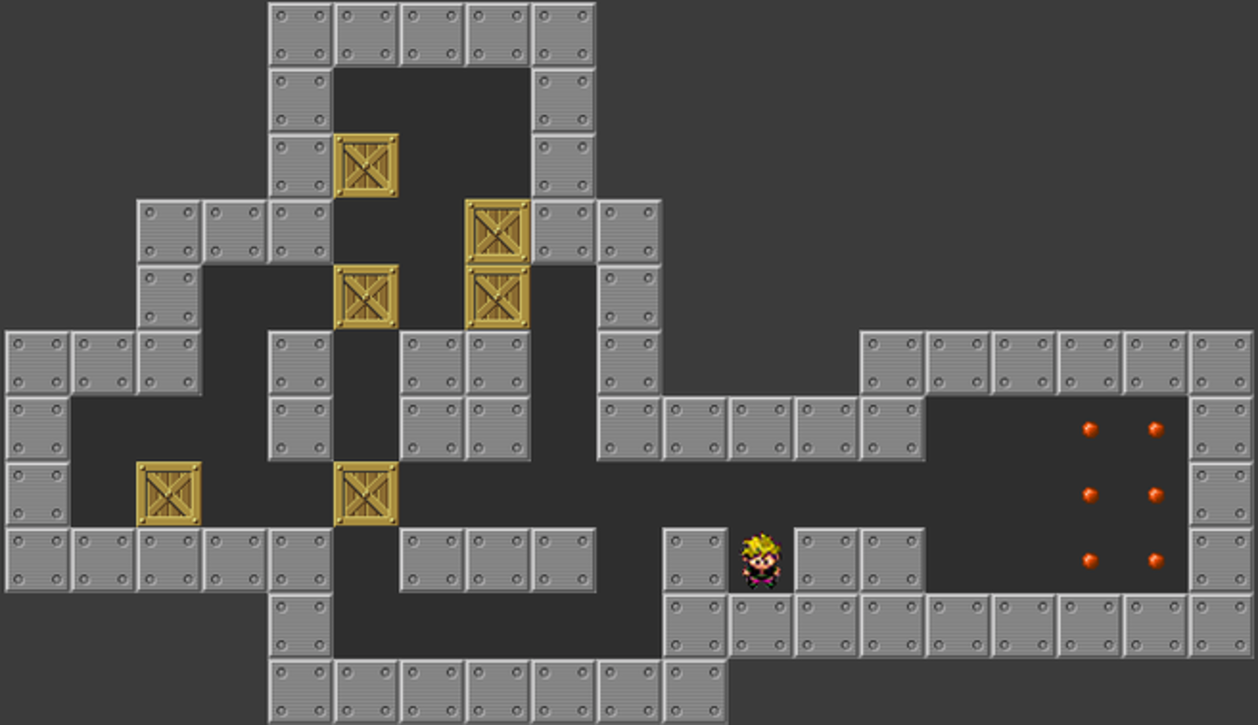
\includegraphics[scale=0.2]{SokobanLevel1}
\caption{First of the Classical Sokoban Levels}
\label{fig:1}
\end{figure}
Figure \ref{fig:1} illustrates the first Sokoban level of the original set of levels. The game is played on a board that can be modelled as a two-dimensional grid. The squares can either be floor or wall squares. Some floor squares are marked as goals and the same number of floor squares contain boxes. The player pushes boxes around this modelled warehouse, trying to cover the marked goal fields (targets) with one of the boxes. For that the player can move one step at a time into one of the four directions \textit{up}, \textit{down}, \textit{left} and \textit{right}. When the player moves onto a box's position the box is pushed one field into the direction of the move. There can never be multiple boxes on one field, neither can there be a box where there is no field. A \textit{solution} to a level is a sequence of moves that leaves a box on each target.
In many of the levels created to this date, the warehouse has a lot of small passageways and very intricate designs. In this thesis I will look at more open level designs, e.g. rectangular levels.
Sokoban is a very difficult planning problem for multiple reasons. There are a lot of possibilities to create a deadlock (a gamestate from which no solution can be found), the branching factor is large and the optimal solution can be very long \cite{BoteaHeuristicsVsPlanning}.
\chapter{Related Work}
\paragraph{Complexity:} Gordon Wilfong published in 1991 that all motion planning problems with moving obstacles are NP-hard \cite{WilfongNPhard}. He proved this by reducing $3$-$Sat$ to such a problem. The question whether Sokoban is PSPACE-complete remained open until 1997, when Joseph C. Culberson published his paper "Sokoban is PSPACE-complete" \cite{PSpaceComplete}. He found a transformation algorithm to transform an LBA into a level of Sokoban, with the solution to the level having a number of steps in $\Theta (|w|+t(|w|))$, where $w$ is the input and $t(|w|)$ is the amount of transitions the LBA made.
\paragraph{Approaches:} There are loads of different researches regarding approaches to Sokoban. I decided which to show. Botea et al. found out that heuristics, while significantly improving chess AI, do not seem to help for planning the soko puzzle \cite{BoteaHeuristicsVsPlanning}. Planning would be a better approach. So to get there and create good plans like humans would, the solver will start meta-reasoning by recognizing rooms and tunnels. Then using those rooms and tunnels to create a plan where first a way is found to bring the crates from the room where theyre at to the target room. Then another plan is made to organize crates in a room.
\paragraph{Macromoves:} Macromoves are a planning strategy that is so successful it is implemented in several good Sokoban solvers. The best example would be Rolling Stone, an excellent Sokoban solver, with a lot of optimizations implemented. One of the optimizations is the possibility to create macromoves for tunnels to reduce all states in the tunnel to one or two, reducing the search space severely.
\begin{figure}[ht]
\centering
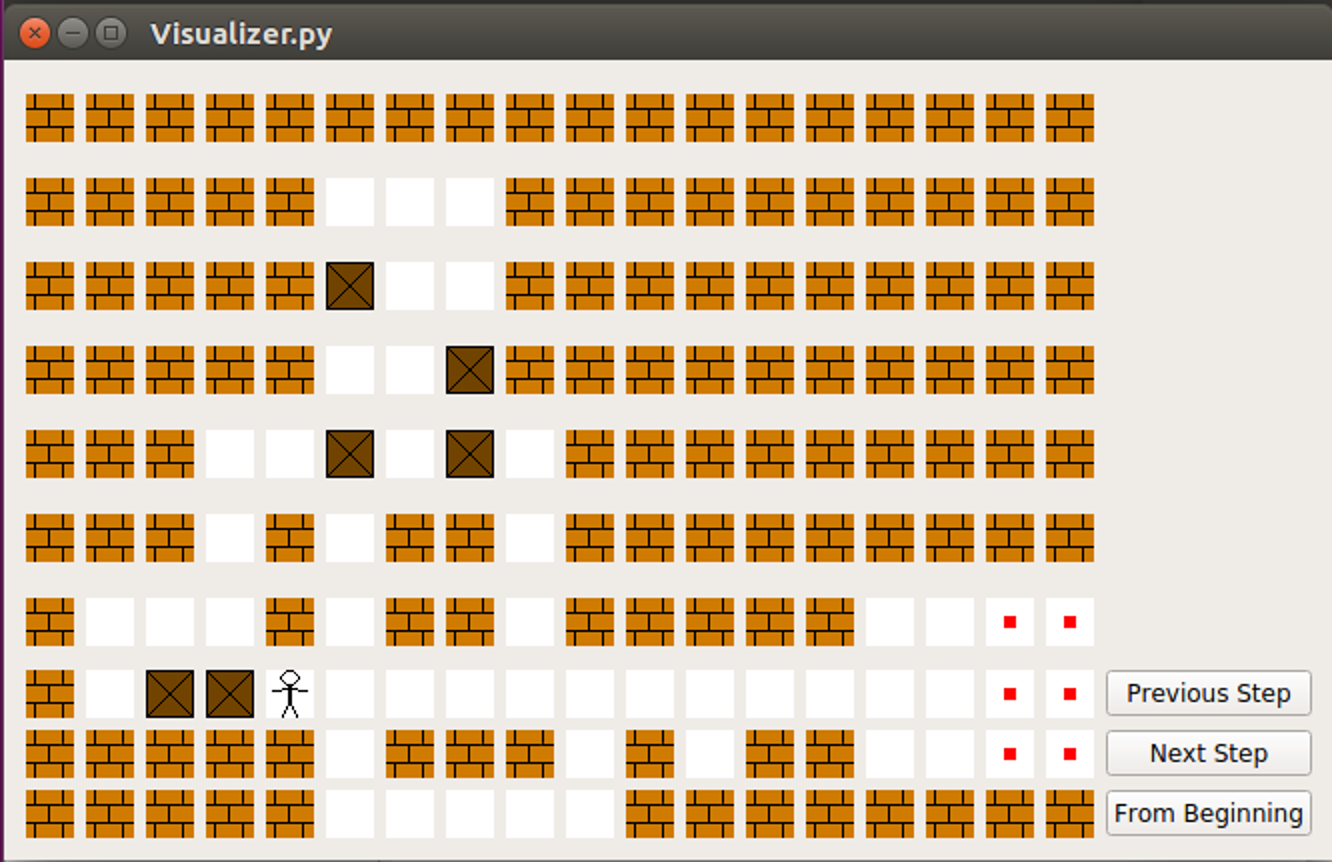
\includegraphics[scale=0.2]{flipped,deadlockexample}
\caption{Deadlock example}
\label{fig:2}
\end{figure}
\begin{figure}[ht]
\centering
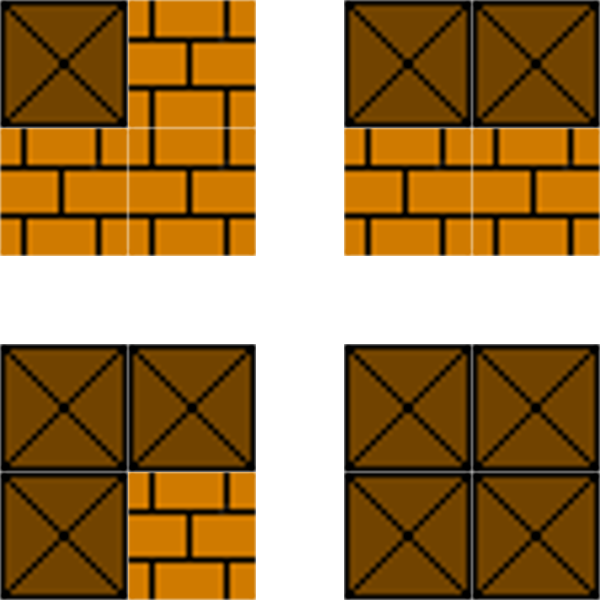
\includegraphics[scale=0.2]{deadlocktypes}
\caption{Deadlock types}
\label{fig:3}
\end{figure}
\paragraph{Deadlock Detection:} Deadlocks are states from which no solution can be found. A trivial example for a deadlock (see Figure \ref{fig:2}) is a box pushed into a corner with no target under it. The box cannot be pulled, so it cannot be recovered from the corner, but to find a solution all boxes have to be covering a target.
Detecting deadlocks the moment they appear is a very powerful optimization, for the reason that huge parts of the search tree can be eliminated early on, without further looking into them. The problem with this strategy is that deadlocks can be very hard to detect, e.g. when they consist of multiple boxes blocking each other in some kind of tunnelsystem. Deadlocks are easier to detect and remove from the search tree when the domain is restricted. When looking at levels with a rectangular shape there are four common deadlocks, cp. Fig. \ref{fig:3}.
\paragraph{Relevance Cutting:} A basic AI to solve a planning problem like Sokoban will look at all possible ways to move around the level, but some of those are dubious but legal or just plain irrelevant. In a lot of cases those dubious ways do not lead to an optimal solution, but of course a problem can be constructed where the optimal solution can only be found when looking at those dubious cases. So Junghanns and Schaeffer tried to teach their AI meta-reasoning to give it the ability to know when to look at those dubious ways and when to ignore them. This they did by creating an influence measurement and only taking moves that are influenced by prior moves, to prevent actions that are disembodied from all prior moves. This is used in the popular Sokoban solver Rolling Stone which has an excellent record in solving Sokoban problems.
\chapter{My Work}
In my work I decided to research Sokoban planning with Answer Set Programming (ASP), a logic programming system designed to return answer sets to queries \cite{LifschitzASP}. I created different basic encodings and optimizations in a modular fashion. Those I will present to you in this chapter. Additionally I created a level portfolio, corresponding to different qualitative properties, e.g. level dimensions or number of boxes, and quantitative properties e.g. a seperation of the level into a zone where all the boxes are placed and a zone where all the targets are placed. The levels have two different types of structures. The first type is a rectangular level with the X and Y dimension differing by 1. The second type is created by connecting 2x2 fields at their edges, see \ref{fig:levelCrooked}.
%. But instead of Prolog ASP is capable of producing answer sets to a query
\cite{BoteaHeuristicsVsPlanning} \cite{Dor1999SOKOBANAO} \cite{Froleyks2017UsingAA} \cite{SokoRelevanceCuts}
\section{Encodings}
In the following, I will present the fact format and the first encodings I used to approach Sokoban solving in the input language of the ASP grounder gringo 3 \cite{Potassco}.
\subsection{Fact Format}
\begin{figure}[ht]
\centering
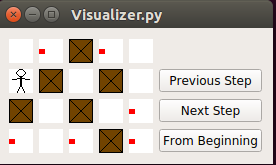
\includegraphics{Visualizer}
\caption{Instance 5x4 with 6 boxes}
\label{fig:levelVis}
\end{figure}
\lstinputlisting{../InstancesClean/Inst-A-Z20-6Halle.lp}
\begin{lstlisting}[caption={Fact Format of my third level},label=lst:lvl1]
\end{lstlisting}
For illustration consider the level shown in Figure \ref{fig:levelVis}. The corresponding fact representation can be seen in Listing \ref{lst:lvl1}. The board size is fixed by the constants $dimX$ and $dimY$ and the origin (1,1) is in the top left corner. The positions of player and boxes are stored in the at/3 predicate. Here the first argument represents the identifier. A zero stands for the player, while all boxes have numbers greater than zero. The second and third argument are the X and Y coordinates, signifying the initial position of the object. For instance init(at(0,1,2)) means the player is at the initial position (1,2). Because I am not exclusively looking at rectangular levels I decided to store all legal fields (meaning fields where a box or player can be placed) by using the predicate field/2. In rectangular levels the legal fields can be defined in one line. Here init(field(1..5,1..4)) (l.4) means the crossproduct of all the numbers in the pools (i.e. (1,1),..,(5,1),(1,2),..,(5,4)).
The goal of the level is given in the target/2 predicate. Each coordinate given by the two arguments of a target/2 instance has to be covered by a box in the final gamestate to solve this level.
Finally the constant horizon stores the information how many steps are needed to successfully satisfy the level. This horizon was determined by using the incremental encoding in section \ref{IncEnc}.
\subsection{Plain Encoding}
\lstinputlisting{../EncodingsClean/SokobanPlainEncoding.lp}
\begin{lstlisting}[caption={Plain Encoding},label=list:PlainEnc]
\end{lstlisting}
The plain encoding seen in listing \ref{list:PlainEnc} uses a strategy common in ASP planning. A choice rule picks the moves (l.6) and the succeeding states are derived from those by using effect and frame axioms (ll.8-11).
In the first few lines basic information is created, namely a $time/1$ predicate for each timestep (l.1), a $dir/2$ predicate for each of the four possible directions to move in (l.3) and an $at/4$ predicate to set the initial positions of objects as their position at time T=0.
Additionally the encoding needs integrity constraints to ensure that the plans found are legal. There is one in line 13 that ensures that no object can move off the playable area and another in line 14 that prevents two object from being at the some position at the same time.
In the lines 16 and 17 the goal condition is defined. The $box/2$ predicate is only created at the last timestep to specify each box position (X,Y). The constraint in line 17 stipulates that all targets have to have a corresponding box predicate with the same coordinates.
The added directive \textbf{\#show at/4.} in line 21 allows for using clingos output as input to my Visualizer \textit{SokoViz}.
This encoding allows to check for a plan of length equal to the horizon constant. This is of course not always optimal, e.g. when one wants to know a shortest plan to solve a level. To achieve an encoding that is able to, I will take advantage of incremental solving.
\subsection{Incremental Encoding} \label{IncEnc}
\lstinputlisting{../EncodingsClean/SokobanIncEncoding.lp}
\begin{lstlisting}[caption={Incremental Encoding},label=list:IncEnc]
\end{lstlisting}
$clingo$ provides an easy to use built-in incremental solving  and grounding mode. An encoding using the inc-mode can be seen in listing \ref{list:IncEnc}. It is very similar to the plain encoding from listing \ref{list:PlainEnc} in having the same structure of a choice rule picking the moves and effect and frame axioms finding the successive state. This encoding is split into three parts, which is critical for using the inc-mode. The \#program base part has only information that is created in the very beginning and will be unchanged throughout the whole grounding and solving process. This infomation is called \#static. The \#program step(t) part is the part accumulating knowledge, holding rules that will be collected and used for each step t and all following steps. The last part \#program check(t) holds volatile rules which will be checked once and discarded for the next timestep. Those rules are used to check for success and are no help to solving following steps.
There is a minor change in the goal defining lines. In the plain encoding the horizon can be used to check efficiently only for the last timestep. In the incremental encoding I carry the time in the $box/3$ prediate to ensure that the constraint in line 21 only affects the target at time t.

\subsection{Split Encoding}
\lstinputlisting{../EncodingsClean/SokobanSplitEncoding.lp}
\begin{lstlisting}[caption={Split Encoding},label=list:SplitEnc]
\end{lstlisting}
The split encoding uses a technique common in ASP planning. When all coordinates are split into a vertical and a horizontal information the grounder does not have to ground all combinations of coordinates ($X * Y$) but only the sum of coordinates ($X + Y$). This has the advantage of less ground instances, but the disadvantage of a harder solving process. Just compare the ramifications in the plain encoding those in the split encoding. The plain encoding can deal with all ramifications in just three rules, while the split encoding needs ten rules. Obviously when splitting the coordinates into horizontal and vertical the rules deriving the new coordinates have to be twice as many. The other problem is that it is harder to find out whether two objects meet each other at a time. That is why the two frame axioms, signifying that boxes that are not touched do not move, have aggregates (ll.17-20). Those are used for simplifying complex rules; the first rule without the aggregates can be seen in listing \ref{list:BadFrame}.
\lstinputlisting{../EncodingsClean/BadSplitFrameAxiom.lp}
\begin{lstlisting}[caption={Frame Axiom X},label=list:BadFrame]
\end{lstlisting}
The last few changes are a second line for the initial readout of the level in lines 4 and 5, a few updates to the integrity constraints in lines 24 and 25 and a slightly different goal definition using the split coordinates.
%Here is another encoding, following a common ASP planning technique that aims to reduce ground instances. By splitting the horizontal and vertical coordinates, the program does not have to ground all combinations ($dimX * dimY$) of coordinates, but just each coordinate by itself (totaling $dimX + dimY$).% only grounds $(dimX + dimY) * horizon * N$ different positions instead of $dimX * dimY * horizon * N$.

\subsection{Optimizations}

\subsubsection{Deadlock Detection}

\lstinputlisting{../EncodingsClean/Optimizations/ForbiddenFields.optimization.lp}
\begin{lstlisting}[caption={Forbidden Fields},label=list:Forbidden]
\end{lstlisting}

Whenever an AI tries to solve a planning problem with a naive encoding, it does not have the meta reasoning a human would have \cite{BoteaHeuristicsVsPlanning}, \cite{SokoRelevanceCuts}. This means it cannot see whether a move is worthless before it calculates its effect. So it has to play through all possible sequences of moves, even those where the first few moves already destroy any chance to satisfy the level. Those gamestates from which no solution can be reached are called deadlocks. A search tree can be greatly reduced if one were to remove all deadlocked branches. The difficulty is that some deadlocks are very hard to notice and sometimes it takes more time eliminating the deadlock than to explore the search tree without eliminating. This is why my deadlock detection approach removes only deadlocks, that are easy to check for. There are three different approaches I tried to remove deadlocks. The Forbidden Fields optimization (listing \ref{list:Forbidden}) works by generating a list of forbidden fields. Those fields are creating deadlocks when the player pushes a box onto them. This approach has the benefit of having a lot of fields that one can exclude from all solution pathways. Those fields are deduced in the \#static part of the program, i.e. they are only grounded once and do not change over the timesteps in a level instance.
The disadvantage of this approach is the rather long time it takes to find all forbidden fields. Furthermore the approach is suited for levels that do not have any restrictions on how they are constructed. As I am looking into levels having a very specific structure (see \ref{IntroStr}), this implementation is not the best approach. In rectangular levels there is an easier way to express a very similar deadlock detection, see next paragraph.

\lstinputlisting{../EncodingsClean/Optimizations/WallBoxTargetCheck.optimization.lp}
\begin{lstlisting}[caption={Deadlock check},label=list:WBT]
\end{lstlisting}

This approach can be seen in listing \ref{list:WBT}. This optimization works best in rectangular levels by simplifying the forbidden check for this special case. The implementaion does not look at tunnels or similar structures but only checks for the outermost lines and rows. When a box is pushed into one of those lines or rows one will not be able to remove it from that line or row. So the idea is to compare the number of boxes in an outermost line or row to the number of targets in it. If the number of boxes exceeds the number of targets the level cannot be satisfied anymore. The result is a very slim check which can help to greatly reduce a search tree.

\lstinputlisting{../EncodingsClean/Optimizations/Clutter.optimization.lp}
\begin{lstlisting}[caption={Clutter},label=list:Clutter]
\end{lstlisting}

My third approach to deadlock detection (see listing \ref{list:Clutter}) recognizes a "clutter" of boxes (see Fig. \ref{fig:clutter}). This is a 2x2 square where each field is either a box or a wall, which would imply that all those boxes would have to stay in their places. In line 8 of the optimization we can see that the box D does not have a target underneath, which qualifies the situation to be a deadlock. This type of deadlock happens a lot in crammed levels with a high box to field ratio. Those very common deadlocks are very important to find and remove to reduce the search tree in those levels efficiently.

\subsubsection{Move Evaluation}

In the following I will show two more optimizations working with move evaluation. This means eliminating movies that will not be relevant for a shortest plan.

\lstinputlisting{../EncodingsClean/Optimizations/MovesOutOfBounds.optimization.lp}
\begin{lstlisting}[caption={Moves out of Bounds},label=list:MOOB]
\end{lstlisting}

The optimization in listing \ref{list:MOOB} is very simple but can remove a lot of moves from grounding, which would be removed after ramifications when checking integrity constraints otherwise. This is more important in levels with a high horizon constant, i.e. a long shortest plan. The optimization works by preventing all moves that would lead the player of the playable area, for instance a move to the left, while the player is at the leftmost position of the level.

\lstinputlisting{../EncodingsClean/Optimizations/NoTakebacks.optimization.lp}
\begin{lstlisting}[caption={No Taking back Moves},label=list:NoTake]
\end{lstlisting}

The last move evaluation seen in listing \ref{list:NoTake} tries to recognize moves that have no effect. This is done by checking for move instances $move(DX,DY,T)$ and $move(-DX,-DY,T-1)$ where no box was moved in timestep T-1. This would imply that the player moved back and forth without actually changing the gamestate, which means the plan is not relevant for finding the shortest plan in the level instance.

\chapter{Discussion}


\section{Experiments and Results}


\chapter{Results}
\section{Tests}
\section{Findings}
\section{Discussion of Results}
compare chapter Related Work with chapter My Work \cite{LifschitzASP}



\begin{thebibliography}{}
\bibitem{LifschitzASP}
Vladimir Lifschitz,
\textit{Answer Set Planning},
ICLP, 1999.

\bibitem{Lifschitz2002AnswerSP}
Vladimir Lifschitz,
\textit{Answer set programming and plan generation},
Artificial Intelligence, 2002, Vol. 138, p.39-54.

\bibitem{LifschitzWhatisASP}
Vladimir Lifschitz,
\textit{What is Answer Set Programming?},
AAAI, 2008.

\bibitem{Gebser2013RicochetRA}
Martin Gebser, Holger Jost, Roland Kaminski, Philipp Obermeier, Orkunt Sabuncu, Torsten Schaub, Marius Thomas Lindauer,
\textit{Ricochet Robots: A Transverse ASP Benchmark},
LPMNR, 2013.

\bibitem{BoteaHeuristicsVsPlanning}
Adi Botea, Martin Müller, Jonathan Schaeffer,
\textit{Using Abstraction for Planning in Sokoban},
Computers and Games, 2002.

\bibitem{Frisch2006PropagationAF}
Alan M. Frisch, Brahim Hnich, Zeynep Kiziltan, Ian Miguel, Toby Walsh,
\textit{Propagation algorithms for lexicographic ordering constraints},
Artificial Intelligence, 2006, Vol. 170, p.803-834.

\bibitem{Dor1999SOKOBANAO}
Dorit Dor, Uri Zwick,
\textit{SOKOBAN and other motion planning problems},
Computational Geometry, 1999, Vol. 13, p.215-228.

\bibitem{Froleyks2017UsingAA}
Nils Christian Froleyks and Tom{\'a}{\^s} Balyo,
\textit{Using an Algorithm Portfolio to Solve Sokoban},
SOCS, 2017.

\bibitem{PSpaceComplete}
Joseph C. Culberson,
\textit{Sokoban is PSPACE-complete},
1997.

\bibitem{SokoRelevanceCuts}
Andreas Junghanns, Jonathan Schaeffer,
\textit{Sokoban: Improving the Search with Relevance Cuts},
Journal of Theoretical Computing Science, 1999, Vol. 252, p.1-2.

\bibitem{SymmetryBreaking}
Brahim Hnich, Zeynep Kiziltan, Toby Walsh,
\textit{Combining Symmetry Breaking with Other Constraints: Lexicographic Ordering with Sums},
ISAIM, 2004.

\bibitem{Potassco}
Martin Gebser, Roland Kaminski, Benjamin Kaufmann, Marius Lindauer, Max Ostrowski, Javier Romero, Torsten Schaub, Sven Thiele,
\textit{Potassco User Guide},
Second Edition, 2015.

\bibitem{WilfongNPhard}
Gordon Wilfong,
\textit{Motion planning in the presence of movable obstacles},
Annals of Mathematics and Artificial Intelligence, 1991.
\end{thebibliography}


\end{document}
